\documentclass[12pt]{article}
\usepackage[top=2in, bottom=1.5in, left=1in, right=1in]{geometry}
\usepackage{pdfpages}
\usepackage{pgfplots}
\usepackage[T1]{fontenc}
\usepackage{graphicx}
\graphicspath{ {images/} }

\begin{document}
\title{NETWORK RELIABILITY API FOR FIREFOX OS\\Improving Efficiency Through Analysis of Network Metadata}
\maketitle
\begin{center}
    \author{John Zeller\\Pok Yan Tjiam\\Jonathan McNeil}
\end{center}
\pagebreak

\tableofcontents
\pagebreak

\section{Introduction}
% Who requested it?
% Why was it requested?
% What is its importance?
% Who was/were your client(s)?
% Who are the members of your team?
% What were their roles?
% What was the role of the client(s)? (I.e., did they supervise only, or did they participate in doing development)

This project was requested by Mozilla, specifically the team working on Firefox OS. Our customer during the course of our project was Dietrich Ayala, a Project Manager working on Firefox OS and a member of the Mozilla family since February 2006. Dietrich's role in our project took many forms, and evolved as what we needed did so. Initially, he helped on board us to the Firefox OS platform, providing us with plenty of documentation to wrap our heads around, and once we have devoured this information, he was quick to setup meeting with members form the Firefox OS networking team. Throughout the year Dietrich was always available via IRC, Skype, Email, and Cell, whenever we needed him. And if he could not answer a question for us, he knew who could.
\\\\
The members of our team were John Zeller, Pok Yan Tjiam, and Jonathan McNeil. John Zeller, having worked with Mozilla for over a year as an intern and contractor, acted as a de facto team lead during the course of the project. Pok Yan Tjiam worked on \_\_\_. Jonathan McNeil worked on \_\_\_.
\\\\
The purpose of this project was to help work towards giving developers a tool that allows them to avoid the typical environment agnostic network request paradigm. As it currently stands, most developers create apps with little to no information about the quality of the network. In their apps, they typically run network requests in a dumb loop, which simply tries continually until the request succeeds. This is wasteful in terms of both battery and data, and overloads an often times already overloaded network.
\\\\
Firefox OS is not a direct competitor to the well known giants in the mobile OS space, but is aimed at being a good solution for the next 4 billion people coming online; the majority of which are coming online in developing countries where network infrastructure is literally decades behind, having a profoundly negative impact on user experience. In many cases poor network conditions can even render some applications non-functional. Aside from out-dated networks, some areas of these developing countries also have unreliable electrical grids, which can make charging a phone take days for many users living with the most unreliable grids. And this problem is only growing worse, at an ever growing pace. In the next 30 days, India alone is expected to account for 5 million new internet users.

\section{Requirements Document}
\subsection{Original}
Here is our original requirements document, featuring the details of our project as we understood them at the time it was written.
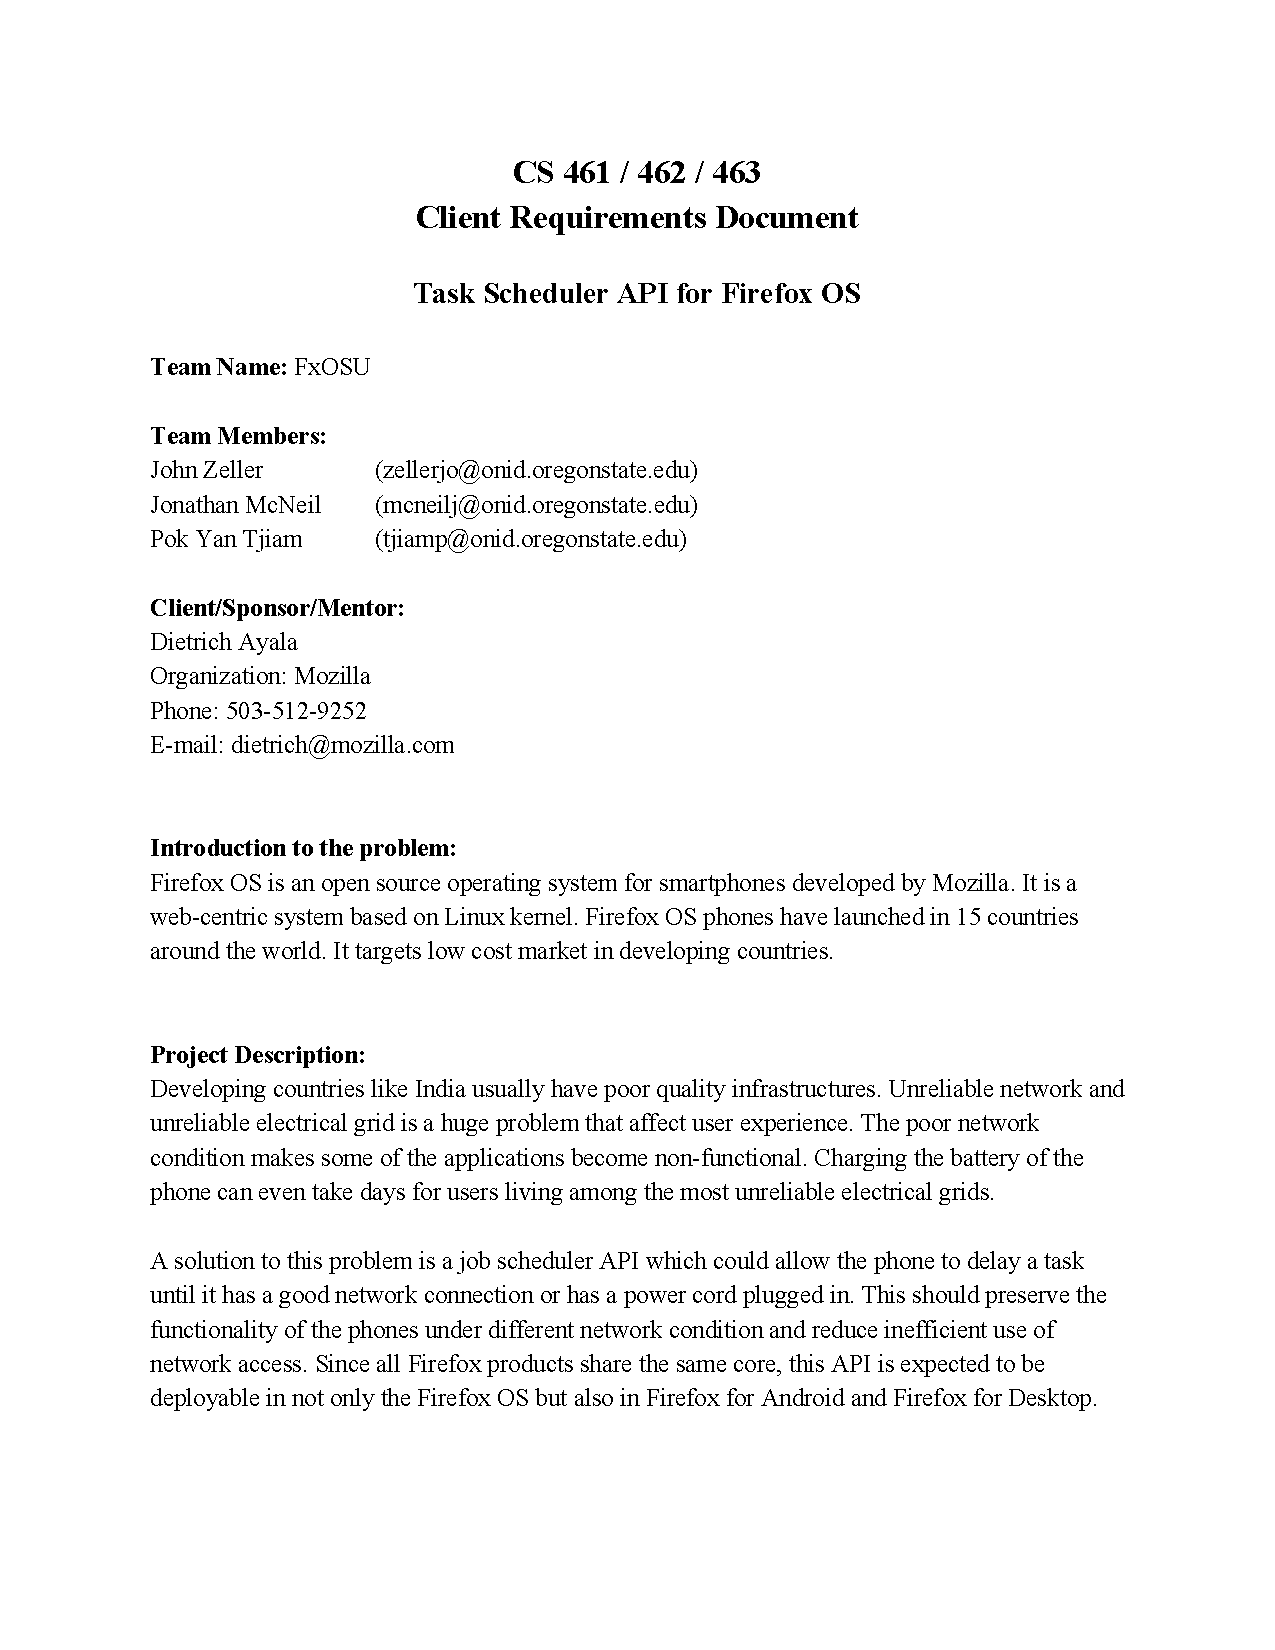
\includepdf[pages={1-8}]{requirementsdoc.pdf}

\subsection{Revisions}
% What new requirements were added? Why? 
% What existing requirements were changed? Why? 
% What existing requirements were deleted? Why? 
% Table featuring changed requirements
	% 1 | Requirement | What happened to it | Comments
% What was the final Gantt chart?

As happens in most projects, requirements change, and ours was no different. Here are the changes that were made to our requirements and why.\\\\
\begin{tabular}{|l|l|l|l|}
\hline
\#  & Requirement 				& What Happened To It 		  & Comments \\ \hline
4	& The API should be written & Modified 					  & The reason for this... \\
	& in C++.					& Changed to "The API should  & \\
	&							& be written in C++ and/or	  & \\
	&							& JavaScript" 				  & \\ \hline
5 	& The API should be callable& Modified 					  & The reason for this... \\
	& by JavaScript executing in& First became "The API should& \\
	& the DOM in a web context. & be callable by JavaScript   & \\
	&							& executing in the window.",  & \\
	&							& Then modified again to 	  & \\
	&							& become "The prototype API   & \\
	&							& should be callable by 	  & \\
	&							& JavaScript executing in a   & \\
	&							& web sandbox." 			  & \\ \hline
6 	& The prototype API should  & Removed 				 	  & The reason for this... \\
	& be able to queue tasks. 	& New requirement was "The 	  & \\
	& 						 	& prototype API should be able& \\
	&							& be able to access data on   & \\
	&							& the battery level of the    & \\
	&							& device in order to determine& \\
	&							& if a task should be 		  & \\
	&							& executed." 				  & \\ \hline
7 	& The prototype API should  & Removed				 	  & The reason for this... \\
	& be able to prioritize		& New requirement was "The 	  & \\
	& tasks in the queue based	& protoype API should be able & \\
	& on network, battery and 	& to access data on the 	  & \\
	& system data.				& charging state of the device& \\
	&							& in order to determine if a  & \\
	&							& task should be executed."   & \\ \hline
\end{tabular}
\pagebreak

\begin{tabular}{|l|l|l|l|}
\hline
\#  & Requirement 				& What Happened To It 		  & Comments \\ \hline
8 	& The prototype API should	& Modified 					  & The reason for this... \\
	& be developer configurable,& Changed to "The prototype   & \\
	& to provide a force		& API should be developer 	  & \\
	& execution of a task after	& configurable, to provide a  & \\
	& a period of time.			& level of certainty about 	  & \\
	&							& network quality."			  & \\ \hline
9 	& The prototype API should  & Modified 				      & The reason for this... \\
	& be able to function  	   	& Changed to "The prototype   & \\
	& without error on Firefox  & API should be able to 	  & \\
	& OS, Firefox for Android,	& function without error on   & \\
	& and Firefox for Desktop.	& Firefox for Desktop."		  & \\ \hline
10 	& The API should be able to & Modified 				      & The reason for this... \\
	& access data on the quality& Changed to "The prototype   & \\ 
	& of the network in order to& API should be able to access& \\
	& determine if a task should& latency-related network     & \\
	& be executed.				& information to determine if & \\
	&							& a task should be executed." & \\ \hline
16 	& The API should be able to & Removed					  & The reason for this... \\
	& queue and postpone tasks	& New requirement was "The API& \\
	& from being dispatched.	& should be able to access 	  & \\
	&							& latency-related network 	  & \\
	&							& information to determine if & \\
	&							& a task should be executed." & \\ \hline
17 	& The API should be able to & Removed 					  & The reason for this... \\
	& prioritize queued tasks 	& New requirement was "The API& \\
	& based on accessible data  & should take into account the& \\
	& about the device and the  & type of network connection, & \\
	& environment.				& whether it be wifi, cellular& \\
	&							& data, etc."				  & \\ \hline
18	& The API should have a 	& Removed					  & The reason for this... \\
	& mechanism for dispatching & New requirement was "The API& \\
	& queued tasks.				& should be able to access 	  & \\
	&							& data about recent tx/rx 	  & \\
	&							& data."					  & \\ \hline
\end{tabular}
\pagebreak

\begin{tabular}{|l|l|l|l|}
\hline
\#  & Requirement 				& What Happened To It 		  & Comments \\ \hline
19 	& The API should be  	    & Modified 					  & The reason for this... \\
	& developer configurable, to& Changed to "The API should  & \\
	& prioritize application 	& be developer configurable,  & \\
	& specific tasks.			& to provide a level of 	  & \\
	&							& certainty about network 	  & \\
	&							& quality."					  & \\ \hline
20 	& The API should be  	    & Removed					  & The reason for this... \\
	& developer configurable,   & New requirement was "The 	  & \\
	& to provide a force  	    & prototype API should be able& \\
	& execution of a task after & to access data about recent & \\
	& a period of time.			& tx/rx data to determine if a& \\
	&							& task should be executed."	  & \\
	&							& Then, the requirement was   & \\
	&							& modified to become "The 	  & \\
	&							& prototype API should be able& \\
	&							& to see if the device has an & \\
	&							& internet connection to 	  & \\
	&							& determine if a task should  & \\
	&							& be executed."				  & \\ \hline
\end{tabular}
\pagebreak

Here is the final Gaant chart for how our project timeline actually turned out.

\begin{figure}[h!]
  \centering
	\includegraphics[scale=0.7]{finalgaant.png}
  \caption{The final Gaant chart for how our project timeline actually turned out.}
\end{figure}


\section{Weekly Team Blog Posts}
\begin{enumerate}
	\item These should be formatted nicely and clearly distinct from one another.
\end{enumerate}

\section{Project Poster}
This is the final project poster that we used when demoing our project at the Engineering Expo.

% \includepdf[pages={1}]{poster.pdf}


\section{Project Documentation}
\begin{enumerate}
    \item How does your project work?
    	\subitem What is its structure?\\
    	\subitem What is its Theory of Operation?\\
    	\subitem Block and flow diagrams are good here. 
    \item How does one install your software, if any?
    \item How does one run it?
    \item Are there any special hardware, OS, or runtime requirements to run your software?
    \item Any user guides, API documentation, etc. 
\end{enumerate}

\section{Learning New Technology}
\begin{enumerate}
    \item What web sites were helpful? (Listed in order of helpfulness.)
    \item What, if any, reference books really helped?
    \item Were there any people on campus that were really helpful? 
\end{enumerate}

\section{What did we learn from all of this?}
\subsection{John Zeller}
\begin{enumerate}
    \item What technical information did you learn?
    \item What non-technical information did you learn?
    \item What have you learned about project work?
    \item What have you learned about project management?
    \item What have you learned about working in teams?
    \item If you could do it all over, what would you do differently? 
\end{enumerate}

\subsection{Pok Yan Tjiam}
\begin{enumerate}
    \item What technical information did you learn?
    \item What non-technical information did you learn?
    \item What have you learned about project work?
    \item What have you learned about project management?
    \item What have you learned about working in teams?
    \item If you could do it all over, what would you do differently? 
\end{enumerate}

\subsection{Jonathan McNeil}
\begin{enumerate}
    \item What technical information did you learn?
    \item What non-technical information did you learn?
    \item What have you learned about project work?
    \item What have you learned about project management?
    \item What have you learned about working in teams?
    \item If you could do it all over, what would you do differently? 
\end{enumerate}

\section{Appendix I}
\begin{enumerate}
	\item Essential Code Listings. You don't have to include absolutely everything, but if someone wants to understand your project, there should be enough here to learn from. If you worked within a larger project, something like a patch file might be a good way to go. 
\end{enumerate}

\section{Appendix II}
\begin{enumerate}
	\item Anything else you want to include. Photos, etc. 
\end{enumerate}

\end{document}